\documentclass[conference]{IEEEtran}

\usepackage{graphicx}
\graphicspath{{figures/}}
\DeclareGraphicsExtensions{.pdf,.jpeg,.png,.eps}
\usepackage[cmex10]{amsmath}
\usepackage{amsfonts}
\usepackage{amssymb}
\usepackage{algorithmic}
\usepackage{array}
\usepackage{mdwmath}
\usepackage{mdwtab}
\usepackage{eqparbox}
\usepackage{caption}
\usepackage{subcaption}
%\usepackage[tight,footnotesize]{subfigure}
%\usepackage[caption=false,font=footnotesize]{subfig}
%\usepackage{stfloats}
\usepackage{fixltx2e}
\usepackage{url}
\usepackage[a4paper,bindingoffset=0.2in,left=1in,right=1in,top=1in,bottom=1in,footskip=.25in]{geometry}

\bibliographystyle{plain}
\DeclareGraphicsExtensions{.pdf,.jpeg,.png,.eps}
\graphicspath{{figures/}}

% Math definitions
\newcommand{\norm}[1]{\left\Vert#1\right\Vert}
\newcommand{\abs}[1]{\left\vert#1\right\vert}
\newcommand{\set}[1]{\left\{#1\right\}}
\newcommand{\To}{\longrightarrow}
\newcommand{\Ker}{\textup{Ker}}
\newcommand{\Img}{\textup{Img}}
\newcommand{\diag}{\textup{diag}}
\newcommand{\circulant}{\textup{circ}}
\newcommand{\bcf}{\;\mbox{\boldmath ${\cal F}$\unboldmath}}
\def\Vec#1{\!\!\hbox{$#1$\kern-0.38em\lower0.85em\hbox{$\vec{}\,$}}\,}%
\newcommand{\bbm}{\begin{bmatrix}}
\newcommand{\ebm}{\end{bmatrix}}
\newcommand{\mbf}[1]{\mathbf{#1}}
\newcommand{\mbs}[1]{{\boldsymbol{#1}}}
\newcommand{\mbb}[1]{{\mathbb{#1}}}
\newcommand{\mc}[1]{\mathcal{#1}}
\newcommand{\argmin}{\operatornamewithlimits{argmin}}
\newcommand{\argmax}{\operatornamewithlimits{argmax}}
\newcommand{\expect}{\operatornamewithlimits{\mbb{E}}}

\begin{document}

\title{Sparse Planning Graphs for \\ Information Driven Exploration}

% This block only works in IEEE mode
\author{\IEEEauthorblockN{Erik Nelson, Vishnu Desaraju, John Yao}
 \IEEEauthorblockA{The Robotics Institute\\
   Carnegie Mellon University\\
   Pittsburgh, PA 15217\\
   \small \{\texttt{enelson}, \texttt{rajeswar}, \texttt{johnyao}\}\texttt{@cmu.edu}}}

\date{}

\maketitle

\begin{abstract}
  \boldmath
  \blindtext
\end{abstract}

\section{Introduction}
\label{sec:introduction}

% Motivation
Exploration is a key capability that enables robotic vehicles to operate in
unknown environments. In this project we develop an active perception policy
for robotic exploration. Active perception exploration formulations
choose control actions which optimize an information-theoretic objective
function such as Shannon's mutual information or entropy
\cite{bourgault2002information, stachniss2005information} over the robot's map,
given a sensor measurement model. Other common exploration techniques, such as frontier
exploration \cite{}, use geometric reasoning to infer explorative paths.
While these strategies work well in practice, they operate on a
maximum likelihood estimate of the map, and apply heuristics to determine the most uncertain
locations in the environment. In contrast, active perception strategies do not utilize
geometric or maximum likelihood assumptions, and instead interpret the map as a binary
random variable, choosing actions which directly minimize the random variable's uncertainty.
Additionally, information-based exploration methods easily extend to 3D
configuration spaces, a benefit which is not shared by frontier methods.
Julian et al. prove that maximizing mutual information between a
robot's map and expected future map naturally yields explorative behaviors
\cite{julian2013mutual}.

% Overview of our approach
Active perception formulations seek to optimize information-theoretic
objectives. While this optimization is real-time for short planning horizons,
these metrics are often expensive to compute online, requiring double
integration over possible future robot states and measurements, or Monte Carlo sampling
from the distribution of measurements. These expensive per-pose computations inhibit
online dense evaluation over a configuration space. In this project, we aim to develop an
efficient active perception exploration strategy which evaluates the
information-theoretic objective in a sparse, but well-chosen set of poses across the
configuration space. This strategy evaluation the objective function
a limited number of times, while still generating paths that sufficiently explore the space.

% Overview of RRT
To achieve real-time active perception exploration, we use a Rapidly-Exploring Random Tree
(RRT) to generate sets of dynamically feasible actions over a finite planning horizon
\cite{Kuwata09_TCST}. RRT planners trade trajectory optimality for efficiency, allowing for evaluation
of many potential future locations in the configuration space during a single planning
step. In addition, RRT planners are anytime, and generate potential trajectories
for a pre-specified amount of time before evaluating the most optimal sampled trajectory. Our
strategy evaluates each RRT leaf-node using the information-theoretic objective function,
and stores the resulting reward in the tree. After planning for a specified
amount of time, the maximum reward leaf-node is chosen as the optimal location to
visit, and the RRT is traversed to generate a dynamically feasible trajectory to
that location.

% Overview of CSQMI
In addition to the efficiency gains from using an RRT, a recent work by Charrow
et al. \cite{charrow15} has
proposed the Cauchy-Schwarz Quadratic Mutual Information (CSQMI) as an efficient
information-theoretic objective function. CSQMI is theoretically
well-motivated: it is derived from Renyi's Quadratic Entropy, a generalization of Shannon's entropy.
However, in contrast to Shannon's mutual information (which is derived directly
from Shannon's entropy), CSQMI is shown to have superior computational efficiency.

% Results and implementation
The contribution of this work is an exploration framework to enable online exploration using CSQMI in sparse
planning graphs, such as RRTs. We demonstrate an implementation of our approach
in simulation, and provide analysis of experiments in which a mobile ground
robot must explore an unknown space using a laser scanner range sensor. We discuss the
formulation and implementation of the CSQMI metric, RRT, and a controller and
Unscented Kalman Filter (UKF) that were developed to enable trajectory tracking and
state estimation. Finally, we discuss the implementation of these capabilities
on a real ground robot.

% Overview of sections
This paper is structured in the following manner: Section~\ref{sec:occupancy_grid_mapping}
gives a brief overview of occupancy grid mapping which is necessary for the CSQMI
information metric. Section~\ref{sec:information_theoretic_objective}
details the CSQMI information-theoretic cost objective and its similarities to
Shannon's mutual information. Section~\ref{sec:measurement_model} discusses the
measurement model that was chosen to evaluate expected future measurements.
Sections~\ref{sec:planner} and~\ref{sec:unscented_kalman_filter} cover the RRT and UKF formulations
used in our implementation. Finally, Sections~\ref{sec:results}
and~\ref{sec:conclusion} give results and analysis of our implementation in
simulation, and describe future work towards implementing our algorithms on a
ground robot.

\section{Occupancy Grid Mapping}
\label{section:occupancy_grid_mapping}

We represent the map as an occupancy grid, which consists of a set of cells: $m = \{m^{i}\}_{i=1}^{N}$.
The probability that an individual cell is occupied is given by $p\left(m^{i} \ \vert \ x_{1:t}, z_{1:t}\right)$, where $x_{1:t}$ denotes the history of states of the vehicle, and $z_{1:t}$ denotes the history of range observations accumulated by the vehicle.
We assume that cell occupancy probabilities are independent of one another: $p\left(m \ \vert \ x_{1:t}, z_{1:t}\right) = \prod_{i} p\left(m^{i} \ \vert \ x_{1:t}, z_{1:t}\right)$.
For notational simplicity we write the map conditioned on random variables $x_{1:t}$ and $z_{1:t}$ as $p_{t}\left(m\right) := p\left(m \ \vert \ x_{1:t}, z_{1:t}\right)$.
Additionally, unobserved grid cells are assigned a uniform prior of being occupied.

We represent the occupancy status of grid cell $m^i$ at time $t$ with a log odds expression
\begin{align}
  l_t &:= \log \frac{p \left( m^i \ \vert \ z_{1:t} \right)}{p \left( \bar{m}^i \ \vert \ z_{1:t} \right)}
\end{align}
, where $\bar{m}^i$ denotes the probability that $m^i$ is unoccupied.
When a new observation $z_t$ is obtained, the log odds update is given by
\begin{align}
  l_t &= l_{t-1} + \log \frac{p\left( m^i \ \vert \ z_t \right)}{p \left( m^i \right)} - \log \frac{p\left( \bar{m}^i \ \vert \ z_t \right)}{p \left(\bar{m}^i \right)}
\end{align}
where the last two terms represent the inverse sensor model.

\section{Information-Theoretic Objective}
\label{sec:information_theoretic_objective}

The goal of active perception exploration is to find a dynamically feasible
sequential set of actions over a time interval, $\tau := t+1,\dots,t+T$, which
enable the robot to explore its environment. We use the criteria that an
explorative action is one that allows the robot to position itself in locations
that generate observations that are informative to the robot's map. Under this
criteria, choosing the optimal exploration action will maximally reduce the
uncertainty in the robot's map. More precisely, an \textit{action} can be defined as a discrete sequence of
states, $x_{\tau} = \left[x_{t+1},\dots,x_{t+T}\right]$. While executing an action,
the robot will obtain a set of measurements $z_{\tau}(x_{\tau}) =
\left[z_{t+1}(x_{t+1}),\dots,z_{t+T}(x_{t+T})\right]$ by sensing from the states
$x_{\tau}$. $z_{\tau}(x_{\tau})$ is modeled as a random variable whose distribution
is parameterized by a deterministic action, $x_{\tau}$. In our formulation, we
choose to select actions from a library of motion primitives, $\mc{X}$, which
are generated by a planner. Under these notations, an explorative planner must
determine $x_{\tau}^{*}$: the action that visits locations which allow the robot
to obtain the set of measurements which maximally reduce uncertainty in its
current map.

To determine $x_{\tau}^{*}$, we follow Charrow et al. \cite{charrow15} and maximize the
Cauchy-Schwarz Quadratic Mutual Information (CSQMI) rate between the current map and the
expectation of future measurements collected along an action, $\text{I}_{\text{CS}}[m; z_{\tau} \vert
x_{\tau}]$.
%
\begin{align}
  \begin{split}
    x_{\tau}^{*}
    &=
    \argmax_{x_{\tau} \in \mc{X}^{T}}
    \frac{\text{I}_{\text{CS}}
      \left[
        m
        ;
        z_{\tau}(x_{\tau})
      \right]
    }
    {R\left(x_{\tau}\right)}
    \label{eq:mutual_information}
  \end{split}
\end{align}
%
Here, $R : \mbb{R}^{\vert x_{\tau} \vert} \rightarrow \mbb{R}^{+}$ computes the
estimated time required to complete action $x_{\tau}$. We choose to maximize
CSQMI as opposed to more common metrics, such as Shannon's mutual information
(MI), due to the property that CSQMI can be computed exactly
in $\mc{O}(N^{2})$, and closely in $\mc{O}(N)$, when $N$ is the number of occupancy
grid cells intersected by all rays in $z_{\tau}$. In contrast,
MI requires averaging many $\mc{O}(N^{2})$ Monte Carlo
samples. The full MI and CSQMI solutions are remarkably similar when computed
over an occupancy grid map, further motivating CSQMI's use. CSQMI between the
map and collection of measurements from $\tau$ is given in \eqref{eq:csqmi}.
%
\begin{align}
  \begin{split}
    &\text{I}_{\text{CS}}
    \left[
      m;
      z_{\tau}
    \right]
    = \\
    &\ -\log
    \frac
    {
      (
      \sum
      \int
      p(m, z_{\tau})
      p(m)
      p(z_{\tau})
      dz_{\tau}
      )^{2}
    }
    {
      \sum
      \int
      p^{2}(m, z_{\tau})
      dz_{\tau}
      \sum
      \int
      p^{2}(m)
      m^{2}(z_{\tau})dz_{\tau}
    }
    \label{eq:csqmi}
  \end{split}
\end{align}
%
where sums are over possible enumerations of $m$, and integrals are over the
space of measurements that can be observed during $\tau$. CSQMI is non-negative,
and maps two random variables to a real valued quantity
which represents the information that one learns about each variable by learning
the other. CSQMI is equal to zero if and only if its arguments are independent.

We represent measurements as $B$-tuple random variables, such that a measurement
$z_{k}^{b}$ captured at time $k \in \tau$ contains $B$ beams. Most occupancy grid
measurement models assume that cells not intersected
by a laser beam are not updated in the map. Let $c$ be the set of cells
intersected by laser beam $z_{k}^{b}$, and let $C = \vert c \vert$. Then
$\text{I}_{\text{CS}}[m; z_{k}^{b}] =
\text{I}_{\text{CS}}[c; z_{k}^{b}]$. Charrow et al. \cite{charrow15} derive a closed form
solution to the CSQMI between
a single laser beam and the robot's map.
%
\begin{align}
  \begin{split}
    \text{I}_{\text{CS}}
    [
      c;
      z_{k}^{b}
    ]
    &=
    \log
    \sum_{l=0}^{C} w_{l}
    \mc{N}(0, 2\sigma^{2}) \\
    &+ \bigg(\log
    \prod_{i=1}^{C}
    (o_{i}^{2} + (1 - o_{i})^{2}) \\
    &\ \ \ \sum_{j=0}^{C}
    \sum_{l=0}^{C}
    p(e_{j})
    p(e_{l})
    \mc{N}(\mu_{l} - \mu_{j}, 2\sigma^{2}) \bigg)\\
    &-2\log
    \sum_{j=0}^{C}
    \sum_{l=0}^{C}
    p(e_{j}) w_{l}
    \mc{N}(\mu_{l} - \mu_{j}, 2\sigma^{2})
    \label{eq:single_beam}
  \end{split}
\end{align}
%
Here, $p(e_j)$ is the probability that the $j$th cell in the raycast $c$ is the
first occupied cell, and $o_i = p(c^{i} = 1)$, the probability that $i$th cell
in the raycast is occupied. Weights $w_{l \in [1, C]}$ can be pre-computed over
the raycast to avoid duplication, and are evaluated as
%
\begin{align}
  \begin{split}
    w_{l} &=
    p^{2}(e_{l})
    \prod_{j=l+1}^{C}
    (o_{j}^{2} + (1 - o_{j})^{2})
  \end{split}
\end{align}
%
By assuming that the resolution of the occupancy grid is greater than the
variance of the range sensor, which is typically the case in occupancy grid
mapping scenarios, and by assuming that Gaussians approach zero with growth in $\vert \mu_{l} -
\mu_{j} \vert$, one may assert that the inner sum in the double sum terms is
only non-zero when $l$ is close to $j$. In other words, the $\mc{O}(C^2)$ double
sum terms can be reduced to $\mc{O}(C)$ complexity by assuming
%
\begin{align}
  \begin{split}
    \sum_{j=0}^{C}
    \sum_{l=0}^{C}
    \alpha_{j, l}
    &\approx
    \sum_{j=0}^{C}
    \sum_{l=j-\delta}^{j+\delta}
    \alpha_{j, l} \\
    \sum_{j=0}^{C}
    \sum_{l=0}^{C}
    \beta_{j, l}
    &\approx
    \sum_{j=0}^{C}
    \sum_{l=j-\delta}^{j+\delta}
    \beta_{j, l}\\
  \end{split}
\end{align}
%
where $\delta \ll C$, and $\alpha_{j,l}$ and $\beta_{j, l}$ are the weighted Gaussian terms inside
of the double sums in \eqref{eq:single_beam}. Our simulator and robot's
laser scanners have $\sigma \approx 0.1$ cm, and use occupancy grid sizes of
$10.0$ cm, allowing us to choose $\delta = 1$ with minimal loss of information.


\section{Measurement Model}
\label{sec:measurement_model}

As explained in Sect.~\ref{section:explorative_information_cost_function}, each future position $x_{j}$ will generate a multi-beam range measurement $z_{j}$. We express each measurement as a $K$-tuple random variable, $z_{j} = \left[z_{j, 1}, \dots, z_{j, K}\right]$, with $z_{j, k} \in \left[z_{min}, z_{max}\right]$. A measurement model is required to sample from the distribution $p(z_{\tau})$. Assuming laser beam independence, $p(z_{\tau})$ can be expressed as a product of the measurement probabilities of individual beams at each timestep over the interval $\tau = t+1:t+T$.
%
\begin{align}
  \begin{split}
    p
    \left(
    z_{\tau}
    \right)
    &=
    \prod_{j=t+1}^{t+T}
    \prod_{k=1}^{K}
    p
    \left(
    z_{j, k}
    \right)
  \end{split}
\end{align}
%
The probability of a single beam measurement can be expressed as a function of the true distance, $r$, to the obstacle.
%
\begin{align}
  \begin{split}
    p
    \left(
    z_{j, k}
    \right)
    &=
    \int_{r}
    p
    \left(
    z_{j, k}
    \ \vert \
    r
    \right)
    p
    \left(
    r
    \right)
    dr
  \end{split}
\end{align}
%
\begin{align}
  \begin{split}
    p
    \left(
    z_{j, k}
    \ \vert \
    r
    \right)
    &=
    \left\{
    \begin{array}{ll}
      \mc{N}(z_{j, k} - r, \sigma_{hit}^{2}) &: z_{min} \le r \le z_{max} \\
            \mc{N}(z_{max}, \sigma_{hit}^{2}) &: z_{max} < r \\
                                            0 &: r < z_{min}
    \end{array}
    \right.
    \label{eq:measurement_model}
  \end{split}
\end{align}
%
where $\mc{N}(x - \mu, \sigma^{2})$ is a one-dimensional Gaussian with mean $\mu$ and variance $\sigma^{2}$. The Gaussian term in Eq.~\eqref{eq:measurement_model} is an approximation for the true distribution, which is a complex function of both beam angle as well as non-axial distance-dependent noise. The environment-dependent distribution $p(r)$ corresponds to the probability that an obstacle intersects a beam at range $r$. We model this as a Poisson binomial distribution with probabilities decaying according to the inverse square of the beam range.

On the interval $\left[z_{min}, z_{\max}\right]$, $p(z_{j, k})$ reduces to a Gaussian convolution with $p(r)$ over $r$, which can be computed in $O(n \log n)$ operations with a Fast Fourier Transform. This computation can be reduced to $O(n)$ by assuming that $\sigma_{hit}$ of the range sensor is much smaller than the resolution of the map.

The distribution $p(r)$ represents the probability that the first obstacle along a ray originating at the sensor is found at distance $r$. $p(r)$ can be expressed as a generalization of the geometric distribution for independent, but not identically distributed (i.n.i.d.) Bernoulli trials.
%
\begin{align}
  \begin{split}
    p(r = i)
    &=
    p_{t}(m^i)
    \prod_{j=1}^{i-1}
    \left(
      1 - p_{t}(m^{j})
    \right)
    \\
    &=
    p_{t}(m^i)
    \left(
      \frac{1}{p_{t}(m^{i-1})} - 1
    \right)
    p(r = i - 1)
  \end{split}
\end{align}


\begin{figure}
  \centering
  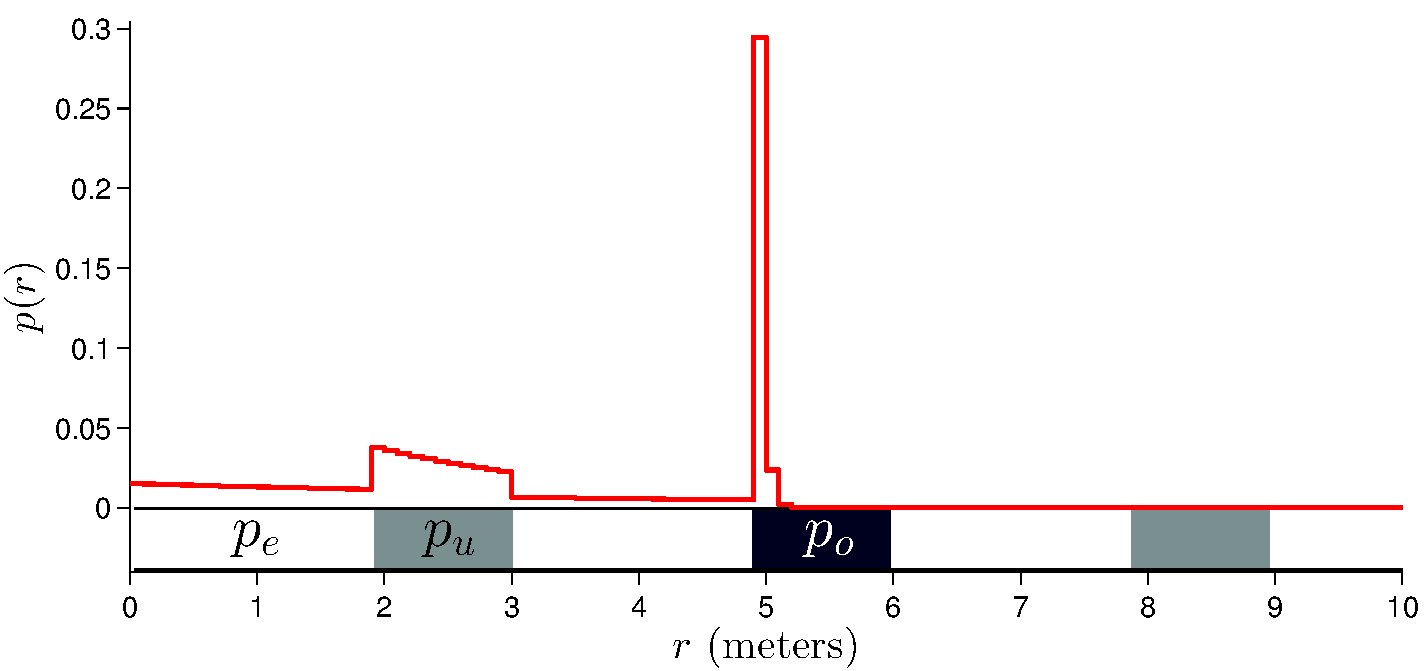
\includegraphics[width=1.0\textwidth]{meas_model.pdf}
  \caption{The distribution $p(r \ \vert \ m)$ over a depicted 1-dimensional map with resolution $\Delta r = 0.1$ m, and $p_{e} = 0.01$, $p_{o} = 0.92$, $p_{u} = 0.05$. \label{fig:measurement_model}}
\end{figure}


\section{Closed Loop RRTs}
\label{sec:planner}

To make use of this information cost function to guide exploration, we consider a sampling-based planning approach that can evaluate the predicted information gain throughout the environment. In addition, we wish to use the occupancy grid that is being updated online (as described in Sect.~\ref{section:occupancy_grid_mapping}) to guide the vehicle around obstacles in the environment. The rapidly-exploring random tree (RRT) algorithm is well suited to planning paths through these types of large environments, and works as follows.
The planner starts from the vehicle's current state and samples a point $x$ in the environment. Using the occupancy grid, we can reject samples that lie in cells with a sufficiently high probability of being occupied. If the sample is valid, we find the closest node in the tree of paths (initially just the vehicle state), where closeness is measured in terms of Euclidean distance, and add a new edge to the tree connecting the sample point to the nearest node.
Then a new sample is drawn and the process repeats to grow a tree of path segments through the environment. This tree-growing process terminates after a specified time, and the minimum cost path is returned.

Figure~\ref{fig:} shows snapshots of the system planning through the environment while updating the occupancy grid. The edges in the tree are smooth since they are generated by forward simulating the closed-loop vehicle dynamics toward the sample point, resulting in a variant of the RRT algorithm known as Closed-loop RRT (CL-RRT)~\cite{Kuwata09_TCST}. This approach is traditionally used to ensure dynamic feasibility and dense collision checking. However, the forward simulation also means we have full state information for the system at the end of each segment. This allows us to evaluate the predicted information gain at that point and assign a corresponding cost to candidate trajectory.

To change CL-RRT from a goal-directed planner to an exploration-driven planner, we first define the sampling distribution to be a Gaussian centered about the root of the tree, with no bias toward any direction (unlike standard sampling-based planners that will sample the goal some small probability). We also define the cost of each branch segment to just be the information metric computed at its endpoint (as opposed to a more traditional setup where the cost is the total distance traveled from the root plus a cost to go based on an admissible heuristic, such as Euclidean distance to a goal). Finally, since there is no goal to guide the selection of the best branch from the tree, we simply select the branch with the minimum cost endpoint in the entire tree. This enables the planner to compute paths that aim to maximize the predicted information gain.

Define $\mathcal{X}_\text{free}$ to be the space spanned by the unoccupied cells in the occupancy grid.

\begin{algorithm}
\caption{CL-RRT: Tree Expansion}
\label{alg:clrrt_expansion}
\begin{algorithmic}[1]
\State Sample point $x_s$ from the environment
\State Select min-cost node from $n$ nearest in tree
\State $k \gets 0$
\State $\hat{x}(t+k) \gets $ last state at n
\While{$\hat{x}(t+k) \in \mathcal{X}_\text{free}(t+k)$ and $\hat{x}(t+k) \neq x_s$}
	\State Compute control input to drive system to $x_s$
	\State Forward simulate system dynamics
	\State Compute next state $\hat{x}(t+k+1)$ from propagation model
	\State $k \gets k+1$
\EndWhile
$N \gets r_final$
\For{each feasible node $N$ produced}
	\State Update cost estimates for $N$
	\State Add $N$ to tree
\EndFor
\end{algorithmic}
\end{algorithm}

\section{State Estimation}
\label{sec:state_estimation}

State estimation addresses the problem of determining the robot's pose in the environment given noisy sensor observations.
This state estimation pipeline's pose output is a superior alternative to directly feeding in exteroceptive sensor observations to the controller and planner.
In this section, we present an Unscented Kalman Filter for fusing inertial measurement unit (IMU) and localization observations for a 2D robot.

\subsection{Process Model}
The vehicle state $\mbf{x}$ consists of the global position $\mbf{p} = \left[ p_x \ p_y \right]^T$, global heading angle $\theta$, global velocity $\mbf{v} = \left[ v_x \ v_y \right]^T$, IMU angular velocity bias in the $z$-direction $b_\omega$ and IMU linear acceleration biases in the $x$- and $y$-directions $\mbf{b}_a = \left[ b_{ax} \ b_{ay} \right]^T$.
%
\begin{align}
  \dot{\mbf{p}} &= \mbf{v} \\
  \dot{\theta} &= \omega - b_\omega - n_\omega \\
 \dot{\mbf{v}} &= \mbf{C}(\theta) \left( \mbf{a} - \mbf{b}_a - \mbf{n}_a \right) \label{eq:vdot} \\
\dot{b}_\omega &= n_{b\omega} \label{eq:bomegadot} \\
  \dot{\mbf{b}}_a &= \mbf{n}_{ba} \label{eq:badot}
\end{align}
%
The IMU measurements are comprised of the $z$-direction angular velocity $\omega$ as well as the body frame $x$- and $y$-direction linear accelerations $\mbf{a} = \left[ a_x \ a_y \right]^T$.
Both measurements are modelled as being corrupted by additive Gaussian white noise and a random walk bias driven by Gaussian white noise \eqref{eq:bomegadot}, \eqref{eq:badot}.
\begin{align}
  \mbf{n} &= \bbm \mbf{n}_a \\ n_\omega \\ \mbf{n}_{ba} \\ n_{b\omega} \ebm \sim \mathcal{N}(\mbf{0}, \mbf{Q}) \label{eq:processnoise} \\
  \mbf{Q} &= \text{diag}\{ \sigma_a^2, \sigma_a^2, \sigma_\omega^2, \sigma_{ba}^2, \sigma_{ba}^2, \sigma_{b\omega}^2 \} \label{eq:Q}
\end{align}
Since the IMU measurements are in the body frame, we use a 2$\times$2 rotation matrix $\mbf{C}(\theta)$ to rotate them into the global reference frame \eqref{eq:vdot}.
Each component of the noise vector in \eqref{eq:processnoise} is assumed to be independent, and their corresponding covariance sigma values are chosen by offline sensor characterization tests \eqref{eq:Q}.

\subsection{Correction Model}
The laser scans are used to construct a map of the environment, and a grid-based localization algorithm is used to compute the global pose (position and heading) of the vehicle with respect to the map.
The sensor model for the localization algorithm is given by
\begin{align}
  \mbf{z} &= \bbm \mbf{p} \\ \theta \ebm + \bbm \mbf{C}(\theta) & \mbf{0} \\ \mbf{0}^T & 1 \ebm \mbf{w} \label{eq:observationmodel} \\
  \mbf{w} &\sim \mathcal{N}(\mbf{0}, \mbf{R} ) \label{eq:obsnoise}
\end{align}
The observation noise covariance matrix $\mbf{R}$ \eqref{eq:obsnoise} is computed by fitting a multivariate Gaussian to the posterior probability grid of the localization algorithm.
Because this covariance is expressed in the scanner frame (assumed to be coincident with the body frame), we rotate its associated noise vector $\mbf{w}$ into the world frame in \eqref{eq:observationmodel}.

\subsection{Unscented Kalman Filter}
The nonlinearities introduced by the rotation in the process and correction models motivated the choice of the Unscented Kalman Filter in this project.
For brevity, we omit the complete presentation of all the steps involved in the UKF (we refer the reader to \cite{Julier97_SPIE}).
We apply the process model and correction model equations when the relevant measurement is received by the state estimator.
Outlier exteroceptive observations are rejected by a chi-squared innovation gate.

\section{Results}
\label{sec:results}

\begin{figure*}
  \centering
  \begin{subfigure}{0.47\textwidth}
    \centering
    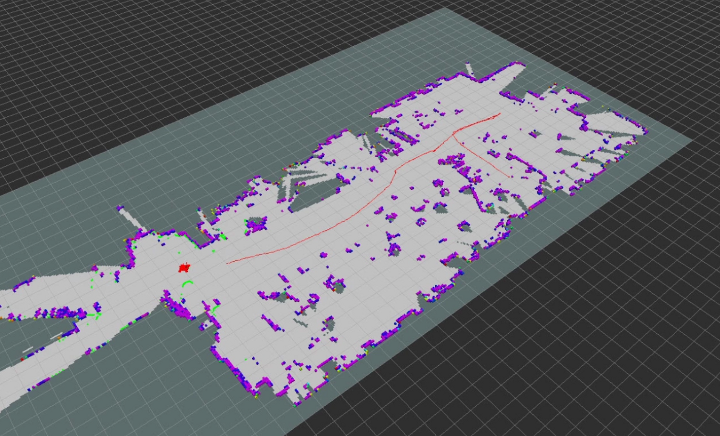
\includegraphics[height=4.3cm]{ground1.png}
    \caption{Map and exploration trajectory\label{fig:ground_bot1}}
  \end{subfigure}
  ~
  \begin{subfigure}{0.47\textwidth}
    \centering
    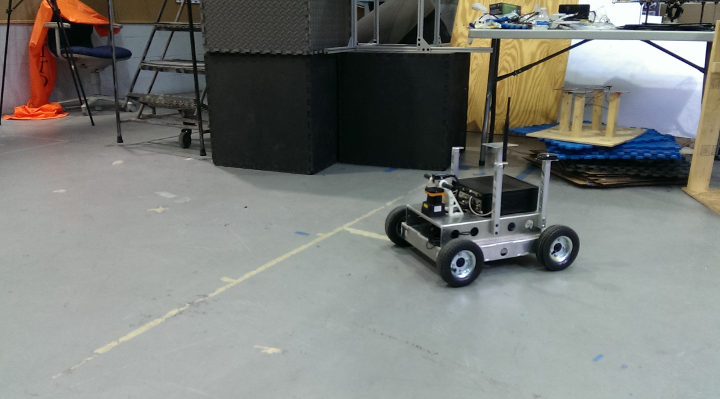
\includegraphics[height=4.3cm]{ground2.png}
    \caption{Ground robot\label{fig:ground_bot2}}
  \end{subfigure}
  \caption{A ground robot exploring and mapping a cluttered environment.\label{fig:ground_bot}}
\end{figure*}


\section{Conclusion and Future Work}
\label{sec:conclusion}

In this work, we have presented a novel approach for information-based exploration and validated performance of this approach using a high-fidelity simulation environment of our ground robot platform. These results demonstrate that this information-based planning strategy is able to accurately and automatically identify regions of the environment that will yield the most information, plan feasible paths to these regions, and successfully explore the environment.

While our approach can be used to successfully produce maps of large environments, it can have difficulty escaping local minima where the RRT's paths do not extend far enough into new unknown territories. In future work, we will adaptively modify the RRT's parameters and planning time to enable consideration of longer trajectories when the map's entropy rate becomes low.

Having verified the exploration strategy in simulation, we would also like to experiment with it using a ground robot (Fig.~\ref{fig:ground_bot2}). We currently have the UKF and SLAM running on the ground robot (see map and state estimate in Fig.~\ref{fig:ground_bot1}), so the next steps would be to transition and integrate the planning and control software. In addition, it would be useful to implement the strategy on aerial robots to see if it easily extends to 6D configuration spaces. 



\bibliography{refs}

\end{document}
